% Wczytanie szablonu
\documentclass[nostrict]{Szablon}

% Definicja dokumentu
\usepackage[unicode=true]{hyperref}
\usepackage{pdfpages}
\usepackage{tabularx}
\newcommand\PDFtitle{Wirtualny escape room z fizyki na poziomie szkoły średniej}
\newcommand\PDFauthors{}
\hypersetup{
  pdftitle={\PDFtitle},
  pdfauthor={\PDFauthors},
}

% Zmiana czcionki dla symulacji maszynopisu (verbatim)
\makeatletter
\renewcommand{\verbatim@font}{\ttfamily\small}
\makeatother

% Część właściwa pracy
\begin{document}
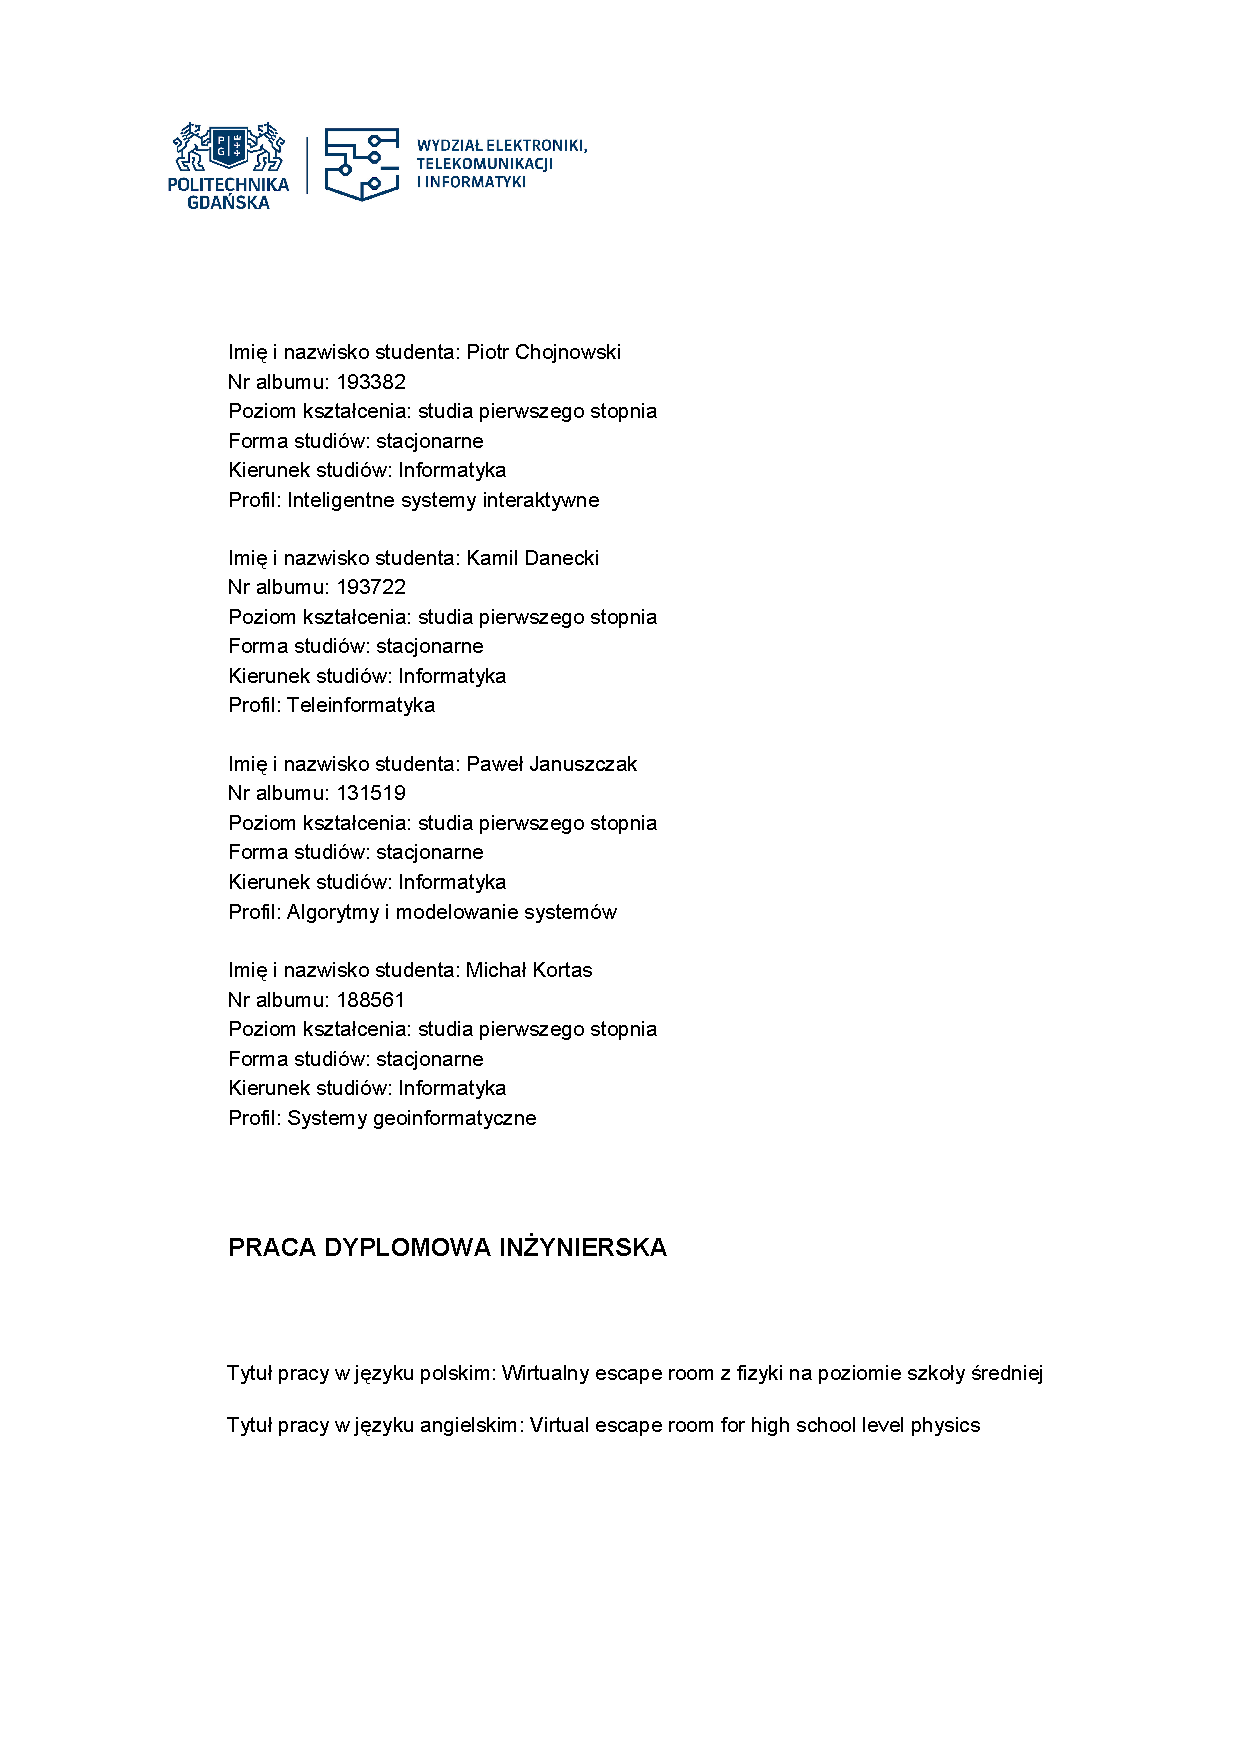
\includepdf[pages={1,2}, scale=1]{StronaTytulowa_193382.pdf}
\chapter*{Streszczenie}
\addcontentsline{toc}{chapter}{Streszczenie}  
Celem tej pracy było stworzenie aplikacji w stylu escape room na system CAVE, służąca jako pomoc naukowa dla uczniów szkół średnich pozwalająca na naukę fizyki przez grę. Aplikacja została stworzona w silniku Unreal Engine 5.5. Gra składa się z 11 pokoi, gdzie każdy pokój mieści w sobie zagadkę na temat jednego działu fizyki. Działy te to: mechanika, mechanika bryły sztywnej, grawitacja i elementy astronomii, drgania, termodynamika, elektrostatyka, prąd elektryczny, magnetyzm, fale i optyka, fizyka atomowa, elementy fizyki relatywistycznej i fizyka jądrowa.

Praca opisuje cały proces tworzenia aplikacji od wstępnych projektów do badań pilotażowych. 

Michał Kortas był odpowiedzialny za organizację zespołu. Jest równierz autorem następujących rozdziałów: 6. Podsumowanie.

Piotr Chojnowski był odpowiedzialny za projekt zagadek z fali i optyki, prądu eltektrycznego oraz elektrostatyki. Jest również autorem następujących rozdziałów: Strzeszczenie, Wykaz skrótów, 3. Technologie, algorytmy i 4. Projekt systemu.

Paweł Januszewski był odpowiedzialny za . Jest równierz autorem następujących rozdziałów: 2. Wprowadzenie do dziedziny.

Kamil Danecki był odpowiedzialny za . Jest równierz autorem następujących rozdziałów: 1. Wstęp i cel pracy.
\newline
\newline
\textbf{Słowa Kluczowe:} escape room, unreal engine, unreal engine 5, gra, wirtualna rzeczywistość
\newline
\newline
\textbf{Dziedzina nauki i techniki, zgodnie z wymogami OECD:} Nauki przyrodnicze, Nauki o komputerach i informatyka

\chapter*{Abstract}
\addcontentsline{toc}{chapter}{Abstract}  

\chapter*{Spis treści}
\addcontentsline{toc}{chapter}{Spis treści}

\tableofcontents

\chapter*{Wykaz ważniejszych oznaczeń i skrótów}
\addcontentsline{toc}{chapter}{Wykaz ważniejszych oznaczeń i skrótów}

\begin{itemize}
    \item CAVE (Cave automatic virtual environment) - jaskinia  rzeczywistości wirtualnej czyli pomieszczenie, którego ściany są ekranami do projekcji stereoskopowej

    \item Escape Room - rodzaj umysłowej gry przygodowej w którym grupa uczestników zostaje zamknięta w specjalnie          przygotowanym pokoju i musi użyć elementów znajdujących się w pokoju, aby rozwiązać szereg zagadek, znaleźć wskazówki i wykonać zadania w celu wydostania się z pokoju w określonym czasie.

    \item FER (Fizyczny Escape Room) - aplikacja wytworzona podczas tworzenia tej pracy 


    \item LZWP (Laboratorium Zanurzonej Wizualizacji Przestrzennej) - Labolatorium znajdujące się na wydziale ETI w Politechnice Gdańskiej

    \item UE5 (Unreal Engine 5) - silnik gier komputerowych, wyprodukowany przez przedsiębiorstwo Epic Games

    \item VR (virtual reality) - obraz sztucznej rzeczywistości stworzony przy wykorzystaniu technologii informatycznej. Polega na multimedialnym kreowaniu komputerowej wizji przedmiotów, przestrzeni i zdarzeń. 

\end{itemize}
\chapter{Wstęp i cel pracy (Kamil Danecki)}
\label{chap:introduction}

Obecnie technologie wytwarzania aplikacji VR rozwijają się w bardzo szybkim tempie. 
Z jednej strony powstają nowe urządzenia pozwalające na jeszcze większą immersję gracza w świat wirtualny, a z drugiej coraz więcej programów umożliwia wykorzystywanie tych urządzeń do produkcji aplikacji końcowych.
Jedną z najbardziej imponujących technologii jest CAVE, czyli sześcienna jaskinia rzeczywistości wirtualnej. 
Jest to pomieszczenie, którego ściany są ekranami do projekcji stereoskopowej. \cite{cave_wiki} 
Jedna z takich jaskiń znajduje się w LZWP na wydziale Elektroniki, Telekomunikacji i Informatyki Politechniki Gdańskiej.

Celem niniejszej pracy inżynierskiej jest wytworzenie aplikacji na CAVE znajdującym się w LZWP na Politechnice Gdańskiej, służącej jako pomoc naukowa dla uczniów szkół średnich, pozwalającej na naukę fizyki przez grę. 
Gatunkiem gry jest escape room, jest to rodzaj gry grupowej, której celem jest rozwiązanie szeregu zagadek.
Ten format gry wykorzystuje przewagę CAVE nad innymi technologiami VR, które pozwalają brać udział w doświadczeniu immersji świata wirtualnego wielu osobom jednocześnie. 
Nie jest to pierwsza implementacja tego typu gry na CAVE, jednak wszystkie poprzednie miały problemy, które w tej pracy postanowiliśmy rozwiązać. 
Problemy te zostały dokładniej opisane w rozdziale drugim.

Oprócz znalezienia rozwiązań dla problemów napotkanych w innych grach tego typu, czymś zupełnie nowym jest tematyka gry - fizyka. Jest to przedmiot, który ze względu na dużą ilość eksperymentów, jakie się podczas jego realizacji przeprowadza, bardzo dobrze się nadaje do wizualizacji w CAVE'ie.
Gra składa się z 11 poziomów, a w każdym z nich jest zagadka z innego działu fizyki - mechaniki, mechaniki bryły sztywnej, grawitacji i elementów astronomii, drgań, termodynamiki, elektrostatyki, prądu elektrycznego, magnetyzmu, fal i optyki, fizyki atomowej, elementów fizyki relatywistycznej i fizyki jądrowej. 
Istotnym aspektem pracy nad aplikacją było opracowanie fabuły gry, która pozwoliłaby uczniom w pełni zanurzyć się w wirtualnym świecie, zamiast postrzegać ją jedynie jako zestaw zadań z fizyki.
Zdecydowaliśmy się na styl fantastycznego średniowiecza, w którym gracze muszą pomóc królestwu ludzi obronić się przed atakiem smoka władającego krainą orków.
Jednocześnie wyjątkową dbałość przykładaliśmy do tego, aby zachować wszystkie walory edukacyjne.

Jako silnik gry wykorzystaliśmy UE (Unreal Engine) firmy Epic Games, Inc. 
Jest to narzędzie umożliwiające tworzenie gier o bardzo realistycznym wyglądzie.
Ta możliwość jest bardzo istotna przy tworzeniu gier aplikacji VR, ponieważ gracze będą widzieli obiekty w znacznie większej skali niż to ma miejsce w standardowych aplikacjach.
W najnowszych wersjach, UE5.x, wtyczki umożliwiające uruchamianie gier na CAVE'ie działają dużo lepiej, co pozwala nam na większy niż kiedykolwiek poziom zaawansowania naszej aplikacji.

Rozdział drugi wprowadza do dziedziny wytwarzania aplikacji rzeczywistości wirtualnej. Przedstawia wybrane przykłady aplikacji już wytworzonych na CAVE i pokazuje,, w jaki sposób nasza aplikacja rozwiązuje problemy widoczne w innych aplikacjach.
W rozdziale trzecim zostały opisane technologie, narzędzia i algorytmy wykorzystane przy realizacji FER.
Rozdział czwarty opisuje projekt systemu. Znajdują się w nim opisy struktury całej aplikacji, jak i szczegółowe opisy każdej z zagadek.
Rozdział piąty przedstawia badania pilotażowe oraz ich wyniki.


\chapter{Przykłady istniejączych rozwiązań}
\label{chap:field}

W rozdziale omówimy istniejące rozwiązania Pokoju Zagadek oraz ich potencjalne zastosowania.

Escape Room ma wiele zastosowań, w zależności od intencji osób biorących w nim udział, może on być dostosowany do celów rekreacyjnych lub edukacyjnych. Pokój Zagadek często zawiera określony temat i historię, wokół której zbudowane są zagadki w pokoju oraz ogólny postęp całego doświadczenia. 
Zagadki mogą być skonstruowane dla jednego uczestnika lub grupy, w celu kooperacji między uczestnikami. Celem Escape Room jest rozwiązanie wszystkich zagadek w odpowiedniej kolejności i ucieczka z pokoju; ucieczka oznacza osiągnięcie końca zabawy.

W wersji rekreacyjnej, Pokój Zagadek może być zbudowany w celu rozrywki grupowej, często grupy znajomych. Współpraca w rozwiązywaniu zagadek oraz radość ze wspólnego sukcesu są często powodem do odwiedzenia tego rodzaju rozrywek. 

W wersji edukacyjnej, Pokój Zagadek jest bardziej wyspecjalizowany, historia jest mniej istotna w tym przypadku, zagadki oraz ich mechanika stanowią główny cel pokoju.
Celem jest nauka poprzez zabawę, przykładem może być pokój o tematyce matematycznej, gdzie zagadki wymagają znajomości matematyki w celu ich rozwiązania, rozwiązanie zagadki utrwala lub przyswaja daną wiedzę dla gracza.

\section{CAVE}
CAVE jest pomieszczeniem, którego ściany są ekranami do projekcji stereoskopowej, zawiera od trzech do sześciu ekranów.
Jaskinia z sześcioma ekranami zwana jest pełną (ekrany tworzą cztery ściany, podłogę oraz sufit), pozwala to na znacznie lepsze wrażenie immersji podczas jej obsługi.
Do poruszania się oraz interakcji z elementami pokoju używamy specjalnego kontrolera zwanego różdżką. Różdżka posiada guziki, które można przypisać do określonych funkcji w zależności od potrzeb użytkownika. Kolejnym elementem kontrolera jest joystick, może on służyć jako jedna z opcji poruszania się po pokoju. Kolejnym sposobem poruszania się jest obracanie pokoju za pomocą przypisanego guzika lub przywrócenie widoku domyślnego w przypadku utraty orientacji.
Kontroler nie jest jedynym sposobem przemieszczania się po pokoju, istnieją dwa sposoby poruszania się w ograniczonej przestrzeni, jaką dysponuje użytkownik. Przemieszczanie się w CAVE wymaga specjalnego obuwia oraz czystości ekranu podłogi w celu uniknięcia uszkodzeń. Pierwszym sposobem jest chodzenie po jaskini, z powodu ograniczonej przestrzeni rozwiązanie to powoduje wiele ograniczeń i wymaga dodatkowej uwagi użytkownika, aby nie uszkodzić monitorów tworzących ściany, jest to natomiast tanie i proste rozwiązanie.
Kolejnym sposobem poruszania się jest sferyczny symulator chodu, jest to przeźroczysta kula, umożliwiająca nieograniczoną nawigację wewnątrz jaskini.


Jaskinia posiada specjalnie zaprojektowany system dźwięku przestrzennego wykorzystujący głośniki zamontowane dookoła pomieszczenia. Istnieje też możliwość wykorzystania słuchawek bezprzewodowych, ogranicza to jednak poczucie swobody użytkownika.

Jaskinia Zanurzenia Wirtualnego stała się popularnym sposobem uczestnictwa w Pokoju Zagadek. W przeciwieństwie do tradycyjnego fizycznego pokoju, gracz może przemieszczać się między wieloma pokojami bez zmiany swojej lokalizacji w CAVE. Dzięki zmianie poziomów jesteśmy w stanie wyspecjalizować zagadki do poszczególnych pokoi, tworząc łańcuch poziomów o określonym rodzaju wyzwań.

Poza rozrywką CAVE posiada wiele różnych zastosowań dla naukowców lub inżynierów, zastosowania te można pogrupować w trzy ogólne kategorie : wirtualne pokazy, wirtualny trening oraz terapia.
Wirtualne pokazy pomagają zaprezentować informacje w sposób unikatowy dla tego środowiska, na przykład przybliżanie lub oddalanie widoku bez konieczności poruszania się, modelowanie w czasie rzeczywistym, zmiana perspektywy za pomocą guzików lub zmiana skali przy bardzo małych lub wielkich elementach.
Prezentacja jest dobrym sposobem pokazania obiektu lub pomieszczenia, które jeszcze nie istnieje, w odpowiedniej skali. Przykładem jest projekt zaprojektowanego budynku w celu jego oceny. Kolejnym rodzajem prezentacji jest wizualizacja naukowa jak na przykład budowa pierwiastków lub materiałów albo wizualizacja wzoru matematycznego.
Wirtualny trening w jaskini może być dostosowany do potrzeb użytkownika bez konieczności fizycznego przemieszczania urządzeń. Trening może służyć do nauki obsługi urządzeń lub szkolenia innych użytkowników za pomocą wirtualnego przykładu.
Trening może pomóc w nauce zasad obsługi różnych urządzeń lub ich naprawy, potencjalne błędy mogą być wyróżnione i poprawione bez ryzyka dla użytkownika oraz ewentualnego uszkodzenia sprzętu. Dla dużych pojazdów, jak statki, trening wirtualny pozwala w prosty sposób nauczyć użytkownika identyfikacji i naprawy usterek.
Terapia wirtualna obejmuje psychologię oraz medycynę. Wirtualna przestrzeń stanowi unikatowe narzędzie dla psychologów przy badaniach i leczeniu fobii takich jak arachnofobia czy akrofobia (lęk wysokości). Dla lekarzy rzeczywistość wirtualna stanowi dobre narzędzie rehabilitacji, tworzenie ćwiczeń dla pacjenta w formie rozrywki zamiast regularnych ćwiczeń. Kolejnym zastosowaniem jaskini w medycynie jest symulowanie operacji bez narażania pacjenta, pozwala to lepiej wyszkolić chirurgów.
CAVE może służyć też do celów naukowych takich jak projekty inżynierskie i magisterskie, przeprowadzanie badań lub analiza zachowań użytkowników przy rozwiązywaniu wyznaczonych zagadek.
Popularnymi dziedzinami do badań w jaskini są na przykład fizyka i matematyka. 



\section{Pokój zagadek w rzeczywistości wirtualnej}
Escape Room wymaga przygotowania pokoju oraz zagadek przed rozpoczęciem gry, wkład pracy przy przygotowaniach jest też obecny podczas kolejnego podejścia do zabawy, przez tę samą lub inną grupę osób. W celu rozwiązania tego problemu można użyć wirtualnej przestrzeni gry, daje to możliwość zmiany elementów pokoju oraz odświeżenia zagadek z minimalnym wkładem pracy.
Dzięki wirtualnemu pokojowi możemy w szybki sposób wymienić rodzaj tematyki, w której gracz bierze udział, dostosowanie pokoju do potrzeb naukowych osoby biorącej udział w rozwiązywaniu zagadek stanowi przewagę nad tradycyjnymi Pokojami Zagadek.

\section{Pokój zagadek o tematyce fizycznej}
Escape Room o tematyce fizycznej jest pokojem skupiającym się na rozwiązywaniu zagadek z różnych dziedzin fizyki, każdy pokój zawiera wyzwania z konkretnego działu fizyki, są one ułożone w sposób wymagający wiedzy o danej tematyce. 


\chapter{Technologie, algorytmy i narzędzia (Piotr Chojnowski)}
\label{chap:algs}

\section{Technologie}
Aplikacja została stworzona na system CAVE. System ten na postać pokoju w którym ściany zastąpione są ekranami do projekcji stereoskopowej. Został on wynaleziony przez Carolinę Cruz-Neira, Daniela J. Sandin i Thomasa A. DeFanti w Uniwersytecie Illinois w Chicago w 1992. Użytkownik jaskini wchodzi do niej w okularach 3D zaopatrzonych w trackery które sprawdzają położenie jego linii wzroku, dzięki czemu obraz może być odpowiednio dopasowany aby stworzyć iluzję głębi obrazu. CAVE w LZWP jest dodatkowo wyposarzony w kontrolery ART Flystick pozwalające na interakcję z wirtualnym środowiskiem.


\section{Narzędzia}
Do produkcji użyliśmy silnika Unreal Engine 5.5 stworzonego przez przedsiębiorstwo Epic Games. Jest to silnik przeznaczony głównie do tworzenia gier 3D. Wybraliśmy go ponieważ zostały stworzone do niego biblioteki pozwalające na proste przenoszenie aplikacji ze środowiska desktopowego na środowisko CAVE.

Użyliśmy 2 bibliotek: nDisplay pozwalającej aplikacji na wyświetlaniu obrazu na klastrze systemu CAVE oraz Dtrack pozwalający na obsługę kontrolerów ART Flystick.

\section{Algorytmy}
\chapter{Projekt systemu (Piotr Chojnowski)}
\label{chap:project}

Projekt ma za cel stworzenie aplikacji wirtualnego escape roomu do nauki fizyki dla szkoły średniej. Poniższy rozdział przedstawia organizacyjne i projektowe założenia stojące za realizacją aplikacji.

\section{Zespół i harmonogram prac}
Zespół projektowy składa się z czterech studentów:

\begin{itemize} 
    \item Michał Kortas -- Kierownik zespołu z doświadczeniem w modelowaniu 3D w środowisku Blender. Posiada również podstawowe doświadczenie z zakresu projektowania gier komputerowych oraz obsługi silnika Unreal Engine.
    \newline
    \item Piotr Chojnowski -- Posiada podstawowe doświadczenie w programowaniu gier komputerowych oraz obsłudze silnika Unreal Engine. Dodatkowo ma umiejętności w tworzeniu tekstur.
    \newline
    \item Kamil Danecki -- Członek koła naukowego VERTEX zajmującego się tworzeniem gier komputerowych. Doświadczenie w projektowaniu gier oraz obsłudze silnika Unreal Engine.
    \newline
    \item Paweł Januszczak -- Posiada podstawowe doświadczenie w projektowaniu gier komputerowych oraz obsłudze silnika Unreal Engine. Znajomość programowania dla środowiska VR.
\end{itemize}
\hfill
\newline
\begin{table}
    \centering
    \begin{tabular}{ |p{3cm}|p{8cm}|  }
     \hline
     \textbf{Miesiąc} & \textbf{Zadania} \\ 
     \hline
     Luty & Ustalenie ogólnych wymagań. \\
     \hline
     Marzec & Analiza narzędzi i dotychczasowych rozwiązań. \newline 
     Projekt pierwszych zagadek. \\   
     \hline
     Kwiecień & Konsultacje z ekspertem. \newline 
     Projekt pozostałych zagadek. \newline
     Stworzenie mechanizmów poruszania się oraz interakcji z otoczeniem.\\ 
     \hline
     Maj & Implementacja zagadek z mechaniki, termodynamiki oraz drgań. \newline
     Wytworzenie potrzebnych modeli 3D do tych zagadek. \\
     \hline
     Czerwiec & Testy w środowisku CAVE. \newline
     Implementacja zagadek z fizyki atomowej oraz prądu elektrycznego. \newline 
     Wytworzenie potrzebnych modeli 3D do tych zagadek. \\  
     \hline
     Lipiec & Implementacja zagadek z fal i optyki oraz elementów fizyki relatywistycznej i fizyki jądrowej. \newline 
     Wytworzenie potrzebnych modeli 3D do tych zagadek. \\ 
     \hline
     Sierpień & Implementacja zagadek z grawitacji i elementów astronomii oraz mechaniki bryły sztywnej. \newline 
     Wytworzenie potrzebnych modeli 3D do tych zagadek. \\ 
     \hline
     Wrzesień & Implementacja zagadek z elektrostatyki oraz magnetyzmu \newline 
     Wytworzenie potrzebnych modeli 3D do tych zagadek. \\ 
     \hline
     Październik & Testy w środowisku CAVE. \newline
     Poprawy w zagadkach. \\ 
     \hline
     Listopad & Poprawki graficzne. \newline
     Testy przeprowadzone przez osoby trzecie. \\ 
     \hline
     Grudzień & Dokończenie dokumentacji. \\
     \hline
    \end{tabular}
    \caption{Harmonogram pracy}
    \label{tab:harmonogram}
\end{table}
    
\section{Specyfikacja wymagań}
Aplikacja ma być grą zespołową w stylu escape room na system CAVE. Ma zawierać co najmniej 11 zagadek - po jednej zagadce z każdej dziedziny fizyki na poziomie szkoły średniej: mechanika, mechanika bryły sztywnej, grawitacja i elementy astronomii, drgania, termodynamika, elektrostatyka, prąd elektryczny, magnetyzm, fale i optyka, fizyka atomowa, elementy fizyki relatywistycznej i fizyka jądrowa.

\section{Ogólna struktura aplikacji}
Aplikacja ma postać 12 pokoi w rozmiarze 3.4m x 3.4m x 3.4m. Pierwszy pokój pełni funkcję menu głównego i wstępu, a każdy pozostały pokój zawiera rozbudowaną zagadkę z jednej z 11 dziedzin fizyki na poziomie szkoły średniej.

\begin{figure}[h!]
    \centering
    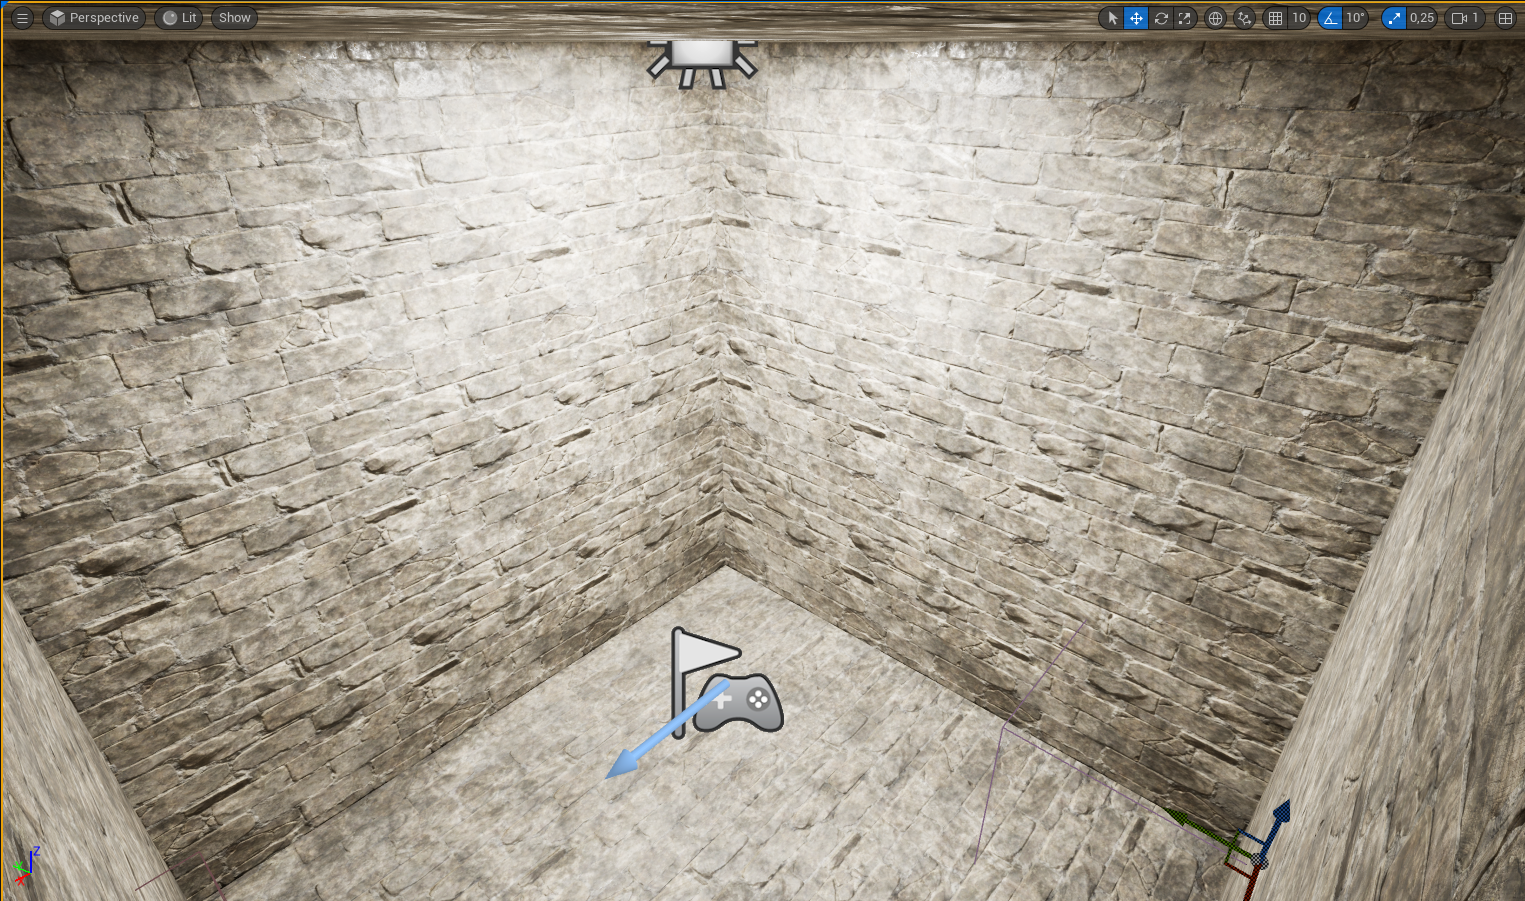
\includegraphics[width=0.6\textwidth]{images/empty_room.png}
    \caption{Przykład pustego pokoju przed implementacją zagadki}
    \label{img:empty_room}
\end{figure}

Gracz zaczyna w pierwszym pokoju. Po rozwiązaniu w nim zagadki przechodzi do kolejnego, wygrywa, gdy ukończy ostatni pokój.\

\section{Projekty zagadek}

Program składa się z 11 różnych zagadek. Zostały one opisane poniżej.

\subsection{Zagadka z mechaniki}
W ramach zagadki z mechaniki gracz będzie musiał użyć drewnianych belek, aby zbudować most, który wytrzyma ciężar przejeżdżającego po nim pojazdu. Na środku pokoju znajduje się miniaturowy wąwóz. Gracz ma limitowaną ilość belek. Gdy pojazd przejedzie na drugą stronę wąwozu, zagadka jest zaliczona jako ukończona.

\subsection{Zagadka z mechaniki bryły sztywnej}
Na środku pokoju znajduje się tarcza zegara ze wskazówką sekund. Zegar jest zatrzymany. Gracz musi właściwie rozmieścić ciężarki, aby zegar zaczął chodzić z odpowiednią prędkością.

\subsection{Zagadka z grawitacji i elementów astronomii}
Aby rozwiązać zagadkę, gracz musi odpowiednio ustawić miniaturowe ciała niebieskie w odpowiednim dystansie i z odpowiednią prędkością, aby ustabilizować układ. Zagadka liczy się jako ukończona, jeżeli układ był stabilny przez ciąg 5-ciu sekund.

\subsection{Zagadka z drgań}
Gracz musi nastroić odpowiednio harfę, aby jej struny wydawały dźwięk o odpowiedniej częstotliwości, a następnie zagrać je w odpowiedniej kolejności, aby odtworzyć melodię składającą się z 5-ciu nut. Zagadka liczy się jako ukończona po zagraniu pełnej melodii.

\subsection{Zagadka z termodynamiki}
Gracz wciela się w kowala, który musi odpowiednio utrzymać temperaturę sztabki żelaza, aby była wystarczająco plastyczna, by uderzając młotem uformować ją w broń. Zagadka liczy się jako zaliczona, gdy broń zostanie uformowana.

\subsection{Zagadka z elektrostatyki}
Zagadka z elektrostatyki stawia gracza w różnych polach elektrostatycznych, gdzie gracz musi dobrać ładunki tak, aby ustabilizować ruch cząsteczek w tych polach. Zagadka liczy się jako ukończona po ustabilizowaniu 3 pól ze zwiększającym się poziomem skomplikowania.

\subsection{Zagadka z prądu elektrycznego}
Zagadka z prądu elektrycznego polega na uzupełnieniu układu elektrycznego, aby dostarczał wystarczające napięcie prądu, jednocześnie nie spalając układu. Gracz dostosowuje parametry elementów, takich jak rezystory, zasilanie i połączenia przewodników. Zagadka liczy się jako ukończona, gdy gracz ukończy dwa układy - pierwszy służy jako poradnik wyjaśniający sterowanie.

\subsection{Zagadka z magneryzmu}
W pokoju znajdują się różnego kształtu magnesy. Gracz musi odpowiednio ustawić linie pól magnetycznych, aby odpowiadały rzeczywistości. Zagadka liczy się jako zaliczona, gdy wszystkie pola są poprawne.

\subsection{Zagadka z fali i optyki}
Zagadka z fali i optyki polega na odpowiednim ustawieniu poprawnych soczewek w lukach w labiryncie na ścianie, tak aby wiązka światła dotarła do jego końca. Przy drugiej ścianie znajduje się stół z różnymi opisanymi soczewkami, które gracz może wybrać. Gracz używa kontrolera, aby przenosić soczewki, które automatycznie wchodzą do luki, gdy są wystarczająco blisko niej. Zagadka liczy się jako ukończona, gdy wiązka światła przejdzie przez labirynt.

\subsection{Zagadka z fizyki atomowej}
Gracz wchodzi w skalę mikro i odpowiednio przesuwa elektrony po orbitach, aby utworzyć z atomów izotopy, a następnie połączyć je w związek. Zagadka liczy się jako ukończona po utworzeniu związku.

\subsection{Zagadka z elementów fizyki relatywistycznej i fizyki jądrowej}
W pokoju znajdują się różne radioaktywne elementy z opisami. Gracz musi odpowiednio je posortować rosnąco zgodnie z ich czasem rozkładu połowicznego. Zagadka liczy się jako zakończona, gdy wszystkie elementy są na ich odpowiednim miejscu. 


\chapter{Implementacja, walidacja i testowanie}
\label{chap:implementation}

\section{Implementacja}

\subsection{Aktorzy}

\subsection{Interfejsy}

\subsection{Modele obiektów}

\subsection{Sceny}

\chapter{Podsumowanie (Michał Kortas)}
\label{chap:summary}

% Bibliografia, ignorujemy overfull box, bo są długie URL
\hfuzz=50pt
\printbibliography[title=\bibliographyname]
\addcontentsline{toc}{chapter}{\bibliographyname}
\hfuzz=0pt

% Wykaz rysunków
\listoffigures
\addcontentsline{toc}{chapter}{\listfigurename}

% Wykaz tabel
\listoftables
\addcontentsline{toc}{chapter}{\listtablename}

\end{document}
